\documentclass[12pt]{article}
\usepackage[margin=2.5cm]{geometry}
\usepackage{enumerate}
\usepackage{amsfonts}
\usepackage{amsmath}
\usepackage{fancyhdr}
\usepackage{amsmath}
\usepackage{amssymb}
\usepackage{amsthm}
\usepackage{mdframed}
\usepackage{graphicx}
\usepackage{subcaption}
\usepackage{adjustbox}
\usepackage{listings}
\usepackage{xcolor}
\usepackage{booktabs}
\usepackage[utf]{kotex}

\definecolor{codegreen}{rgb}{0,0.6,0}
\definecolor{codegray}{rgb}{0.5,0.5,0.5}
\definecolor{codepurple}{rgb}{0.58,0,0.82}
\definecolor{backcolour}{rgb}{0.95,0.95,0.92}

\lstdefinestyle{mystyle}{
    backgroundcolor=\color{backcolour},
    commentstyle=\color{codegreen},
    keywordstyle=\color{magenta},
    numberstyle=\tiny\color{codegray},
    stringstyle=\color{codepurple},
    basicstyle=\ttfamily\footnotesize,
    breakatwhitespace=false,
    breaklines=true,
    captionpos=b,
    keepspaces=true,
    numbers=left,
    numbersep=5pt,
    showspaces=false,
    showstringspaces=false,
    showtabs=false,
    tabsize=1
}

\lstset{style=mystyle}

\begin{document}
\title{CSC148 Worksheet 13 Solution}
\author{Hyungmo Gu}
\maketitle

\section*{Question 1}
\begin{enumerate}[a.]
    \item

    The following diagram tells us the stopping condition occurs when both
    \textit{curr1} and \textit{curr2} is \textit{None}.

    \begin{center}
    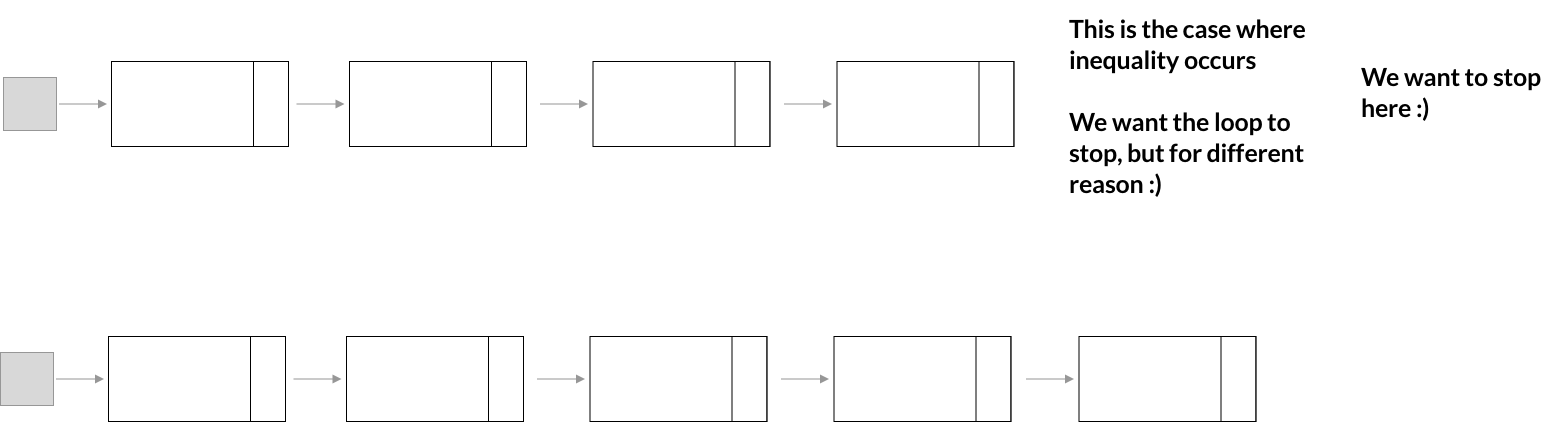
\includegraphics[width=\linewidth]{images/worksheet_13_q1a_solution.png}
    \end{center}

    \bigskip

    Using this fact, the python expression involving \textit{curr1}
    and \textit{curr2} that expresses the stopping condition is

    \bigskip

    \begin{lstlisting}[language=Python]
    (curr1 is not None) and (curr2 is not None)
    \end{lstlisting}

    \item

    Python expression for the while loop condition is

    \begin{lstlisting}[language=Python]
    while (curr1 is not None) and (curr2 is not None):
        ...
    \end{lstlisting}

    \item

    The code for traversing two list is

    \begin{lstlisting}[language=Python]
    while (curr1 is not None) and (curr2 is not None):
        if curr1 is None or curr2 is None:
            return False

        if curr1.item != curr2.item:
            return False

        curr1 = curr1.next
        curr2 = curr2.next
    \end{lstlisting}

    \item

    After the loop ends, we know all items in curr1 and curr2 are identical.

    \item

    Because we know on successful loop termination, all items in curr1 and curr2
    are the same, we can use this information to conclude the two linked lists
    have the same length.

    \item

    The code that should go after the end of while loop is

    \begin{lstlisting}[language=Python]
    return True
    \end{lstlisting}

\end{enumerate}

\section*{Question 2}
\begin{enumerate}[a.]
    \item

    Initially, \textit{curr} and \textit{i} are as follows

    \begin{lstlisting}[language=Python]
    curr = self._first
    i = 0
    \end{lstlisting}

    \item

    The stopping condition for the while loop is

    \begin{lstlisting}[language=Python]
    curr is not None
    \end{lstlisting}

    \bigskip

    Using this fact, we can conclude that the while loop condition is

    \begin{lstlisting}[language=Python]
    while curr is not None:
        ...
    \end{lstlisting}

    \item
    The code for the loop body is
    \begin{lstlisting}[language=Python]
    # 2. If index - 1 != current_index, then continue to next node
    if index - 1 != current_index:
        curr = curr.next
        current_index += 1
        continue

    # 3. If curr.next is none, then let it terminate naturally
    if curr.next is None:
        curr = curr.next
        current_index += 1
        continue

    # 4. If index - 1 == current_index, then return item of curr.next
    return curr.next.item
    \end{lstlisting}

    \item

    After the loop ends, we know \textit{curr} is None and \textit{index == len(self)}.

    \bigskip

    Using this fact, we can write that the post-loop code is

    \begin{lstlisting}[language=Python]
    raise IndexError
    \end{lstlisting}

\end{enumerate}

\bigskip

\begin{lstlisting}[language=Python,caption={worksheet\_13\_q2\_solution.py},captionpos=b]
    def __getitem__(self, index: int) -> Any:
        """Return the item at position <index> in this list.
        Raise an IndexError if the <index> is out of bounds.
        Precondition: index >= 0.

        >>> lst = LinkedList([1, 2, 3])
        >>> print(lst[0])
        1
        >>> print(lst[1])
        2
        >>> print(lst[2])
        3
        >>> print(lst[3])
        Traceback (most recent call last):
            ...
        IndexError
        """

        curr = self._first
        current_index = 0

        # 1. If index == 0 and curr is not none, then return curr.item (edge case)
        if index == 0 and (curr is not None):
            return curr.item

        while curr is not None:
            # 2. If index - 1 != current_index, then continue to next node
            if index - 1 != current_index:
                curr = curr.next
                current_index += 1
                continue

            # 3. If curr.next is none, then let it terminate naturally
            if curr.next is None:
                curr = curr.next
                current_index += 1
                continue

            # 4. If index - 1 == current_index, then return item of curr.next
            return curr.next.item

        raise IndexError
\end{lstlisting}


\end{document}